\documentclass[a4paper,12pt]{article}
\usepackage{amsmath}
\usepackage{amssymb}
\usepackage[polish]{babel}
\usepackage{polski}
\usepackage[utf8]{inputenc}
\usepackage{indentfirst}
\usepackage{geometry}
\usepackage{array}
\usepackage[pdftex]{color,graphicx}
\usepackage{subfigure}
\usepackage{afterpage}
\usepackage{setspace}
\usepackage{color}
\usepackage{wrapfig}
\usepackage{listings}
\usepackage{datetime}
\usepackage{hyperref}


\hypersetup{
  colorlinks   = true, %Colours links instead of ugly boxes
  urlcolor     = blue, %Colour for external hyperlinks
  linkcolor    = blue, %Colour of internal links
  citecolor   = red %Colour of citations
}


\renewcommand{\onehalfspacing}{\setstretch{1.6}}

\geometry{tmargin=2.5cm,bmargin=2.5cm,lmargin=2.5cm,rmargin=2.5cm}
\setlength{\parindent}{1cm}
\setlength{\parskip}{0mm}

\newenvironment{lista}{
\begin{itemize}
  \setlength{\itemsep}{1pt}
  \setlength{\parskip}{0pt}
  \setlength{\parsep}{0pt}
}{\end{itemize}}

\newcommand{\linia}{\rule{\linewidth}{0.4mm}}

\definecolor{lbcolor}{rgb}{0.95,0.95,0.95}
\lstset{
    backgroundcolor=\color{lbcolor},
    tabsize=4,
  language=C++,
  captionpos=b,
  tabsize=3,
  frame=lines,
  numbers=left,
  numberstyle=\tiny,
  numbersep=5pt,
  breaklines=true,
  showstringspaces=false,
  basicstyle=\footnotesize,
  identifierstyle=\color{magenta},
  keywordstyle=\color[rgb]{0,0,1},
  commentstyle=\color{Darkgreen},
  stringstyle=\color{red}
  }
\begin{document}

\noindent
\begin{tabular}{|c|p{11cm}|c|} \hline 
Grupa 1 & Kamil Sacha, Konrad Szwedo & \ddmmyyyydate\today \tabularnewline
\hline 
\end{tabular}

\renewcommand{\lstlistingname}{Listing kodu}

\section*{Zadanie 4 - Rozmycie Gaussa w OpenMP}

Naszym zadaniem laboratoryjnym było napisanie programu wykonującego rozmycie Gaussa, w oparciu o środowisko do zrównoleglania kodu: OpenMP. 
Algorytm Gaussa polega na zastąpieniu pikseli obrazu wejściowego, średnią z obszaru otaczającego ten piksel. W naszym przypadku rozpatrywaliśmy maskę wielkości \(5 \times 5\), czyli do obliczenia musieliśmy znać wszystkie 25 wartości trzech kanałów rozpatrywanego piksela (kanały R - Czerwony, G - Zielony, B - Niebieski). Jako wartość poszczególnego kanału (R, G, B) ustawiamy średnią z całości rozpatrywanego obszaru. 


\subsection*{Podział obrazu pomiędzy wątki}

	Podział wejściowego obrazu jest realizowany automatycznie poprzez zastosowanie poniższej dyrektywy \textbf{\#pragma omp parallel for...}, biblioteka OpenMP rozdziela ilość iteracji pętli odpowiednio do rozmiaru obrazu wejściowego.
	
	\begin{lstlisting}[caption=Główna dyrektywa OpenMP zewnętrznej pętli iterującej po liczbie wierszy.=Pragma]
#pragma omp parallel for private(row, col, i, minus1Row, minus2Row, 
currentRow, plus1Row, plus2Row) num_threads(threads)
\end{lstlisting}	

	Jako zmienne prywatne, czyli te dla których każdy wątek tworzy swoją kopię, zostały ustawione zmienne iteracyjne row, col, i, czyli zmienne oznaczające następująco numer bieżącego wiersza, kolumny, indeks pomocniczy do algorytmu Gaussa. 
	Dodatkowo jako zmienne prywatne oflagowane zostały wskaźniki na 5 wierszy potrzebnych do przyśpieszenia obliczeń, czyli: po dwa wskaźniki na wiersze poprzedzające i następujące oraz wskaźnik na obecny wiersz. 
	Jako obecny wiersz rozumiemy ten wiersz dla którego obliczamy wartość piksela.
	
\subsection*{Algorytm obliczeń}

	Korzystając z biblioteki OpenCV wczytujemy obraz wejściowy, który w pamięci przechowywany jest jako tablica składająca się z wartości każdego kanału piksela.
	 Piksel składa się z 3 kanałów zapisywanych w kolejności odpowiednio (R, G, B).
Każdy kanał reprezentowany jest jako liczba typu \textbf{unsigned char} (w skrócie uchar), czyli liczba typu char bez znaku, która 		     może przechowywać liczby z zakresu [0 - 255]. 
Aby przyśpieszyć odczyt pikseli obrazu wejściowego skorzystaliśmy z metody \textbf{ptr} która zwraca nam wskaźnik na cały wiersz o jaki pytamy. 
Dzięki temu ograniczyliśmy korzystanie z kosztownej obliczeniowo metody \textbf{at} która przelicza za każdym razem wartości wiersza i kolumny na indeks odpowiedniego kanału.

\clearpage
\begin{lstlisting}[caption=Fragment wewnętrznej pętli iterującej po wierszach.=Row pointery]
minus2Row  = my_input_img->ptr<uchar>( row - 2 );
minus1Row  = my_input_img->ptr<uchar>( row - 1 );
currentRow = my_input_img->ptr<uchar>( row     );
plus1Row   = my_input_img->ptr<uchar>( row + 1 );
plus2Row   = my_input_img->ptr<uchar>( row + 2 );
...    
blueTotal  += minus2Row [ blueColIndex ] + minus1Row[ blueColIndex ] +
              currentRow[ blueColIndex ] + plus1Row [ blueColIndex ] +
              plus2Row  [ blueColIndex ];        
...
blueTotal  = round(blueTotal  / 25.0f);
...
my_output_image->at<cv::Vec3b>(row - 2, col - 2) = cv::Vec3b(blueTotal, greenTotal, redTotal);
\end{lstlisting}

\section*{Wyniki i wnioski}

Program zrównoleglony został poprawnie o czym świadczą wykresy czasu wykonania oraz przyśpieszenia w zależności od liczby wątków.
Testy zostały przeprowadzone na serwerze \textbf{cuda.iti.pk.edu.pl}, przy użyciu dostępnego tam 4 rdzeniowego procesora.
Istnieje jeszcze szybsza metoda, dostępu do wierszy obrazu wejściowego, a mianowicie bezpośredni dostęp w którym sami zajmujemy się indeksowaniem wskaźników. Według znalezionych informacji 
\footnote{\href{http://longstryder.com/2014/07/which-way-of-accessing-pixels-in-opencv-is-the-fastest/}
{Which way of accessing pixels in OpenCV is the fastest?}} wynika, że bezpośredni dostęp poprzez wskaźniki jest szybszy od zastosowanej przez nas metody o 18\%. Postanowiliśmy jednak zostawić program w postaci operowania na całych wierszach, gdyż ważniejsze było bezpieczeństwo oraz czytelność kodu.

\begin{figure}

	\begin{center}
 		% GNUPLOT: LaTeX picture with Postscript
\begingroup
  \makeatletter
  \providecommand\color[2][]{%
    \GenericError{(gnuplot) \space\space\space\@spaces}{%
      Package color not loaded in conjunction with
      terminal option `colourtext'%
    }{See the gnuplot documentation for explanation.%
    }{Either use 'blacktext' in gnuplot or load the package
      color.sty in LaTeX.}%
    \renewcommand\color[2][]{}%
  }%
  \providecommand\includegraphics[2][]{%
    \GenericError{(gnuplot) \space\space\space\@spaces}{%
      Package graphicx or graphics not loaded%
    }{See the gnuplot documentation for explanation.%
    }{The gnuplot epslatex terminal needs graphicx.sty or graphics.sty.}%
    \renewcommand\includegraphics[2][]{}%
  }%
  \providecommand\rotatebox[2]{#2}%
  \@ifundefined{ifGPcolor}{%
    \newif\ifGPcolor
    \GPcolortrue
  }{}%
  \@ifundefined{ifGPblacktext}{%
    \newif\ifGPblacktext
    \GPblacktextfalse
  }{}%
  % define a \g@addto@macro without @ in the name:
  \let\gplgaddtomacro\g@addto@macro
  % define empty templates for all commands taking text:
  \gdef\gplbacktext{}%
  \gdef\gplfronttext{}%
  \makeatother
  \ifGPblacktext
    % no textcolor at all
    \def\colorrgb#1{}%
    \def\colorgray#1{}%
  \else
    % gray or color?
    \ifGPcolor
      \def\colorrgb#1{\color[rgb]{#1}}%
      \def\colorgray#1{\color[gray]{#1}}%
      \expandafter\def\csname LTw\endcsname{\color{white}}%
      \expandafter\def\csname LTb\endcsname{\color{black}}%
      \expandafter\def\csname LTa\endcsname{\color{black}}%
      \expandafter\def\csname LT0\endcsname{\color[rgb]{1,0,0}}%
      \expandafter\def\csname LT1\endcsname{\color[rgb]{0,1,0}}%
      \expandafter\def\csname LT2\endcsname{\color[rgb]{0,0,1}}%
      \expandafter\def\csname LT3\endcsname{\color[rgb]{1,0,1}}%
      \expandafter\def\csname LT4\endcsname{\color[rgb]{0,1,1}}%
      \expandafter\def\csname LT5\endcsname{\color[rgb]{1,1,0}}%
      \expandafter\def\csname LT6\endcsname{\color[rgb]{0,0,0}}%
      \expandafter\def\csname LT7\endcsname{\color[rgb]{1,0.3,0}}%
      \expandafter\def\csname LT8\endcsname{\color[rgb]{0.5,0.5,0.5}}%
    \else
      % gray
      \def\colorrgb#1{\color{black}}%
      \def\colorgray#1{\color[gray]{#1}}%
      \expandafter\def\csname LTw\endcsname{\color{white}}%
      \expandafter\def\csname LTb\endcsname{\color{black}}%
      \expandafter\def\csname LTa\endcsname{\color{black}}%
      \expandafter\def\csname LT0\endcsname{\color{black}}%
      \expandafter\def\csname LT1\endcsname{\color{black}}%
      \expandafter\def\csname LT2\endcsname{\color{black}}%
      \expandafter\def\csname LT3\endcsname{\color{black}}%
      \expandafter\def\csname LT4\endcsname{\color{black}}%
      \expandafter\def\csname LT5\endcsname{\color{black}}%
      \expandafter\def\csname LT6\endcsname{\color{black}}%
      \expandafter\def\csname LT7\endcsname{\color{black}}%
      \expandafter\def\csname LT8\endcsname{\color{black}}%
    \fi
  \fi
  \setlength{\unitlength}{0.0500bp}%
  \begin{picture}(7200.00,5040.00)%
    \gplgaddtomacro\gplbacktext{%
      \csname LTb\endcsname%
      \put(1078,704){\makebox(0,0)[r]{\strut{} 1000}}%
      \csname LTb\endcsname%
      \put(1078,1111){\makebox(0,0)[r]{\strut{} 1500}}%
      \csname LTb\endcsname%
      \put(1078,1518){\makebox(0,0)[r]{\strut{} 2000}}%
      \csname LTb\endcsname%
      \put(1078,1925){\makebox(0,0)[r]{\strut{} 2500}}%
      \csname LTb\endcsname%
      \put(1078,2332){\makebox(0,0)[r]{\strut{} 3000}}%
      \csname LTb\endcsname%
      \put(1078,2740){\makebox(0,0)[r]{\strut{} 3500}}%
      \csname LTb\endcsname%
      \put(1078,3147){\makebox(0,0)[r]{\strut{} 4000}}%
      \csname LTb\endcsname%
      \put(1078,3554){\makebox(0,0)[r]{\strut{} 4500}}%
      \csname LTb\endcsname%
      \put(1078,3961){\makebox(0,0)[r]{\strut{} 5000}}%
      \csname LTb\endcsname%
      \put(1078,4368){\makebox(0,0)[r]{\strut{} 5500}}%
      \csname LTb\endcsname%
      \put(1078,4775){\makebox(0,0)[r]{\strut{} 6000}}%
      \csname LTb\endcsname%
      \put(1210,484){\makebox(0,0){\strut{} 0}}%
      \csname LTb\endcsname%
      \put(1909,484){\makebox(0,0){\strut{} 2}}%
      \csname LTb\endcsname%
      \put(2608,484){\makebox(0,0){\strut{} 4}}%
      \csname LTb\endcsname%
      \put(3307,484){\makebox(0,0){\strut{} 6}}%
      \csname LTb\endcsname%
      \put(4007,484){\makebox(0,0){\strut{} 8}}%
      \csname LTb\endcsname%
      \put(4706,484){\makebox(0,0){\strut{} 10}}%
      \csname LTb\endcsname%
      \put(5405,484){\makebox(0,0){\strut{} 12}}%
      \csname LTb\endcsname%
      \put(6104,484){\makebox(0,0){\strut{} 14}}%
      \csname LTb\endcsname%
      \put(6803,484){\makebox(0,0){\strut{} 16}}%
      \put(176,2739){\rotatebox{-270}{\makebox(0,0){\strut{}Średni czas wykonania [ms]}}}%
      \put(4006,154){\makebox(0,0){\strut{}Ilość wątków}}%
    }%
    \gplgaddtomacro\gplfronttext{%
      \csname LTb\endcsname%
      \put(5816,4602){\makebox(0,0)[r]{\strut{}Czas wykonania}}%
    }%
    \gplbacktext
    \put(0,0){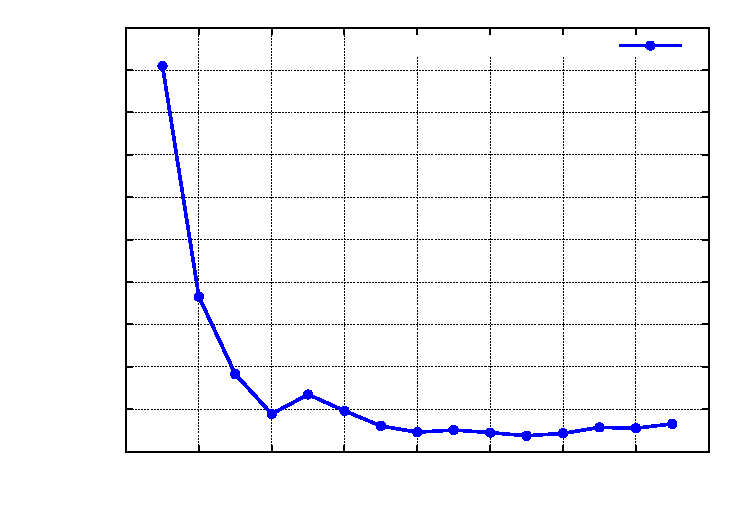
\includegraphics{wykres_czasu}}%
    \gplfronttext
  \end{picture}%
\endgroup
   		 		
	\end{center}
	
    \caption{Wykres zależności czasu wykonania od ilości wątków.
     Dla obrazu wejściowego '1.jpg' o wymiarach \(24107 \times 4491 \approx 10^9\) pikseli.}
\end{figure}


\begin{figure}

	\begin{center}
 		% GNUPLOT: LaTeX picture with Postscript
\begingroup
  \makeatletter
  \providecommand\color[2][]{%
    \GenericError{(gnuplot) \space\space\space\@spaces}{%
      Package color not loaded in conjunction with
      terminal option `colourtext'%
    }{See the gnuplot documentation for explanation.%
    }{Either use 'blacktext' in gnuplot or load the package
      color.sty in LaTeX.}%
    \renewcommand\color[2][]{}%
  }%
  \providecommand\includegraphics[2][]{%
    \GenericError{(gnuplot) \space\space\space\@spaces}{%
      Package graphicx or graphics not loaded%
    }{See the gnuplot documentation for explanation.%
    }{The gnuplot epslatex terminal needs graphicx.sty or graphics.sty.}%
    \renewcommand\includegraphics[2][]{}%
  }%
  \providecommand\rotatebox[2]{#2}%
  \@ifundefined{ifGPcolor}{%
    \newif\ifGPcolor
    \GPcolortrue
  }{}%
  \@ifundefined{ifGPblacktext}{%
    \newif\ifGPblacktext
    \GPblacktextfalse
  }{}%
  % define a \g@addto@macro without @ in the name:
  \let\gplgaddtomacro\g@addto@macro
  % define empty templates for all commands taking text:
  \gdef\gplbacktext{}%
  \gdef\gplfronttext{}%
  \makeatother
  \ifGPblacktext
    % no textcolor at all
    \def\colorrgb#1{}%
    \def\colorgray#1{}%
  \else
    % gray or color?
    \ifGPcolor
      \def\colorrgb#1{\color[rgb]{#1}}%
      \def\colorgray#1{\color[gray]{#1}}%
      \expandafter\def\csname LTw\endcsname{\color{white}}%
      \expandafter\def\csname LTb\endcsname{\color{black}}%
      \expandafter\def\csname LTa\endcsname{\color{black}}%
      \expandafter\def\csname LT0\endcsname{\color[rgb]{1,0,0}}%
      \expandafter\def\csname LT1\endcsname{\color[rgb]{0,1,0}}%
      \expandafter\def\csname LT2\endcsname{\color[rgb]{0,0,1}}%
      \expandafter\def\csname LT3\endcsname{\color[rgb]{1,0,1}}%
      \expandafter\def\csname LT4\endcsname{\color[rgb]{0,1,1}}%
      \expandafter\def\csname LT5\endcsname{\color[rgb]{1,1,0}}%
      \expandafter\def\csname LT6\endcsname{\color[rgb]{0,0,0}}%
      \expandafter\def\csname LT7\endcsname{\color[rgb]{1,0.3,0}}%
      \expandafter\def\csname LT8\endcsname{\color[rgb]{0.5,0.5,0.5}}%
    \else
      % gray
      \def\colorrgb#1{\color{black}}%
      \def\colorgray#1{\color[gray]{#1}}%
      \expandafter\def\csname LTw\endcsname{\color{white}}%
      \expandafter\def\csname LTb\endcsname{\color{black}}%
      \expandafter\def\csname LTa\endcsname{\color{black}}%
      \expandafter\def\csname LT0\endcsname{\color{black}}%
      \expandafter\def\csname LT1\endcsname{\color{black}}%
      \expandafter\def\csname LT2\endcsname{\color{black}}%
      \expandafter\def\csname LT3\endcsname{\color{black}}%
      \expandafter\def\csname LT4\endcsname{\color{black}}%
      \expandafter\def\csname LT5\endcsname{\color{black}}%
      \expandafter\def\csname LT6\endcsname{\color{black}}%
      \expandafter\def\csname LT7\endcsname{\color{black}}%
      \expandafter\def\csname LT8\endcsname{\color{black}}%
    \fi
  \fi
  \setlength{\unitlength}{0.0500bp}%
  \begin{picture}(7200.00,5040.00)%
    \gplgaddtomacro\gplbacktext{%
      \csname LTb\endcsname%
      \put(682,704){\makebox(0,0)[r]{\strut{} 0}}%
      \csname LTb\endcsname%
      \put(682,1722){\makebox(0,0)[r]{\strut{} 1}}%
      \csname LTb\endcsname%
      \put(682,2740){\makebox(0,0)[r]{\strut{} 2}}%
      \csname LTb\endcsname%
      \put(682,3757){\makebox(0,0)[r]{\strut{} 3}}%
      \csname LTb\endcsname%
      \put(682,4775){\makebox(0,0)[r]{\strut{} 4}}%
      \csname LTb\endcsname%
      \put(814,484){\makebox(0,0){\strut{} 1}}%
      \csname LTb\endcsname%
      \put(1242,484){\makebox(0,0){\strut{} 2}}%
      \csname LTb\endcsname%
      \put(1670,484){\makebox(0,0){\strut{} 3}}%
      \csname LTb\endcsname%
      \put(2097,484){\makebox(0,0){\strut{} 4}}%
      \csname LTb\endcsname%
      \put(2525,484){\makebox(0,0){\strut{} 5}}%
      \csname LTb\endcsname%
      \put(2953,484){\makebox(0,0){\strut{} 6}}%
      \csname LTb\endcsname%
      \put(3381,484){\makebox(0,0){\strut{} 7}}%
      \csname LTb\endcsname%
      \put(3809,484){\makebox(0,0){\strut{} 8}}%
      \csname LTb\endcsname%
      \put(4236,484){\makebox(0,0){\strut{} 9}}%
      \csname LTb\endcsname%
      \put(4664,484){\makebox(0,0){\strut{} 10}}%
      \csname LTb\endcsname%
      \put(5092,484){\makebox(0,0){\strut{} 11}}%
      \csname LTb\endcsname%
      \put(5520,484){\makebox(0,0){\strut{} 12}}%
      \csname LTb\endcsname%
      \put(5947,484){\makebox(0,0){\strut{} 13}}%
      \csname LTb\endcsname%
      \put(6375,484){\makebox(0,0){\strut{} 14}}%
      \csname LTb\endcsname%
      \put(6803,484){\makebox(0,0){\strut{} 15}}%
      \put(176,2739){\rotatebox{-270}{\makebox(0,0){\strut{}Średnie przyśpieszenie}}}%
      \put(3808,154){\makebox(0,0){\strut{}Liczba wątków}}%
    }%
    \gplgaddtomacro\gplfronttext{%
      \csname LTb\endcsname%
      \put(5816,877){\makebox(0,0)[r]{\strut{}Przyśpieszenie}}%
    }%
    \gplbacktext
    \put(0,0){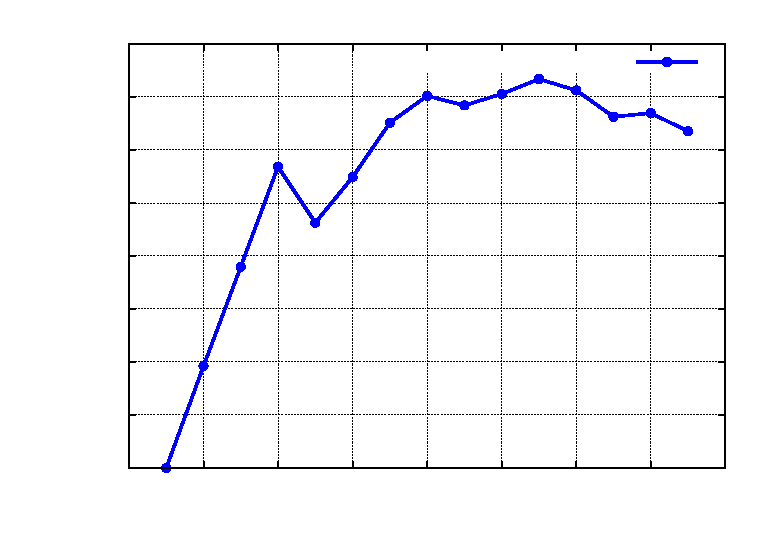
\includegraphics{dane/wykres_przyspieszenia}}%
    \gplfronttext
  \end{picture}%
\endgroup
   		 		
	\end{center}
	
    \caption{Wykres zależności przyśpieszenia od ilości wątków.
     Dla obrazu wejściowego '1.jpg' o wymiarach \(24107 \times 4491 \approx 10^9\) pikseli.}
\end{figure}

\end{document}